\newcommand{\quelle}{%
	\small Quelle:
}

\newcommand{\registered}{\textsuperscript{\textregistered}}

%Einzug bei neuem Absatz auf 0pt Einrücken
%\setlength{\parindent}{0pt}

\chapter{Hardware}


Im Rahmen des Projektes wurden unterschiedlichste Komponenten von verschiedenen Herstellern eingesetzt.
Dieses Kapitel soll einen Überblick über die verwendete Hardware geben.
Darunter einige Eigenschaften und Besonderheiten auf die ggf. in den Nachfolgenden Unterabschnitten näher eingegangen wird.

%----------------------------------------------------------------------------------
\section{Infineon XMC 4700/4800 Relax Kit}
\label{sec:INF XM4700/4800}
Für die Auswertung der verschiedenen Sensoren wurden Mikrocontroller des Herstellers Infineon aus der XMC 4000 Serie genutzt.
Diese werden kurz beschrieben.
Im Anschluss wird auf Probleme mit diesen eingegangen.

\subsection{Allgemeine Beschreibung} 
\paragraph{Hinweis:} Da die Mikrocontroller XMC 4700 und XMC 4800 nahezu identisch sind ist die nachfolgende Beschreibung für beide Controller gültig.
Auch wird zwischen den beiden Relax Kits nicht unterschieden
Auf die Besonderheiten nach dem folgenden Abschnitt eingegangen.

\paragraph{XMC Mikrocontroller:}
Bei dem XMC Relax Kit handelt es sich um eine Entwicklungsplattform für den XMC Mikrocontroller.
Innerhalb des Controllers arbeitet ein ARM\registered Cortex\registered-M4 mit einer Taktfrequenz von 144 MHz.
Dieser bildet die CPU, welche um zahlreiche Schnittstellen erweitert wird.
Als Kommunikationsschnittstellen stehen unter anderem Ethernet, USB,  CAN und USART zur Verfügung.
Für die Erfassung Analogen Signalen stehen mehrere \enquote{Versatile Analog-Digital Converters} (VADC) mit je 8 Kanälen und einer Auflösung von 12-Bit zur Verfügung.
Weiterhin sind Digital-Analog-Konverter(DAC) mit einer Auflösung von 12-Bit integriert.

Eine Besonderheit der XMC 4000 Serie ist das \enquote{Position Interface} (POSIF).
Dieses Modul stellt eine Schnittstelle für die Steuerung von Motoren bereit.
Hierzu kann POSIF wahlweise mit Hall-Sensoren, Drehgebern oder mittels Software versorgt werden.
Aus diesen Sensorinformationen wird im Anschluss ein Steuersignal für die Ansteuerung des Motors generiert.\cite{InfineonTechnologies2016a}
%Hierbei handelt es sich um ein Modul für die Steuerung von verschiedensten Motoren unter Verwendung von Hall-Sensoren, Drehgebern oder externen Steuersignalen. \cite[Kap. 25]{InfineonTechnologies2016}
%ref Reference Manual Chap 25.2.7.1

Eine vollständige Auflistung der enthaltenen Komponenten kann dem Referenzhandbuch \cite{InfineonTechnologies2016} oder der Produkthomepage \cite{InfineonTechnologies2017} entnommen werden .

\paragraph{Relax Kits:}
Infineon stellt, für die Einarbeitung und Tests, kleine Entwicklungsplattformen bereit.
Dabei handelt es sich um Platinen, die bereits mit einem XMC Mikrocontroller und allen dafür notwendigen Bauteilen versehen ist.
Zum Teil sind diese Entwicklungsplatinen für die Aufnahme von sog. Arduino Shields vorgesehen um Modular den Mikrocontroller zu erweitern.
Hier ist jedoch zu beachten, dass nicht jedes Relax Kit alle Erweiterungsplatinen aufnehmen kann.
Für das Aufspielen von Programmen bzw. zum Debuggen verfügen die Relax Kits über eine JTAG Schnittstelle\footnote{Kurzform für Joint Test Action Group und Synonym für IEEE-Standard 1149.1.}.

In Abbildung \ref{fig:XMC4700} ist Beispielhaft eines der Relax Kits dargestellt, die während des Projektes zum Einsatz kamen.
In der Mitte befindet sich der Mikrocontroller. 
Über- und Unterhalb von diesem sind Buchsenleisten für die Aufnahme von Arduino Shields bereits aufgelötet.
Die noch nicht bestückten Lötaugen sind mit dem Controller verbunden und können mit Stift- oder Buchsenleisten versehen werden.
In der linken unteren Ecke ist die JTAG Schnittstelle angebracht, die mittels eines Micor-USB Anschlusses mit einem PC verbunden werden kann. 

\subsection{XMC 4700 Relax Kit 5V}
\label{sec:XMC4700}
Dieses Kit ist für die Verwendung der Arduino Shields vorgesehen.
Da es sich bei der Arduino Plattform um 5 Volt Mikrocontroller handelt sind die Shield vorwiegend auf diese Spannung ausgelegt.
Der XMC arbeitet hingegen mit einem Logikpegel von 3.3 Volt.
Aus diesem Grund hat Infineon für die Digitalen Pins Bidirektionalen Levelshifter verbaut.
Mit diesen werden die 5 Volt Signal auf 3.3 Volt bzw. anderes herum gewandelt.
Dadurch kann eine Vielzahl von Erweiterungsplatinen ohne Änderungen verwendet werden.

\begin{figure}[h]
	\centering
	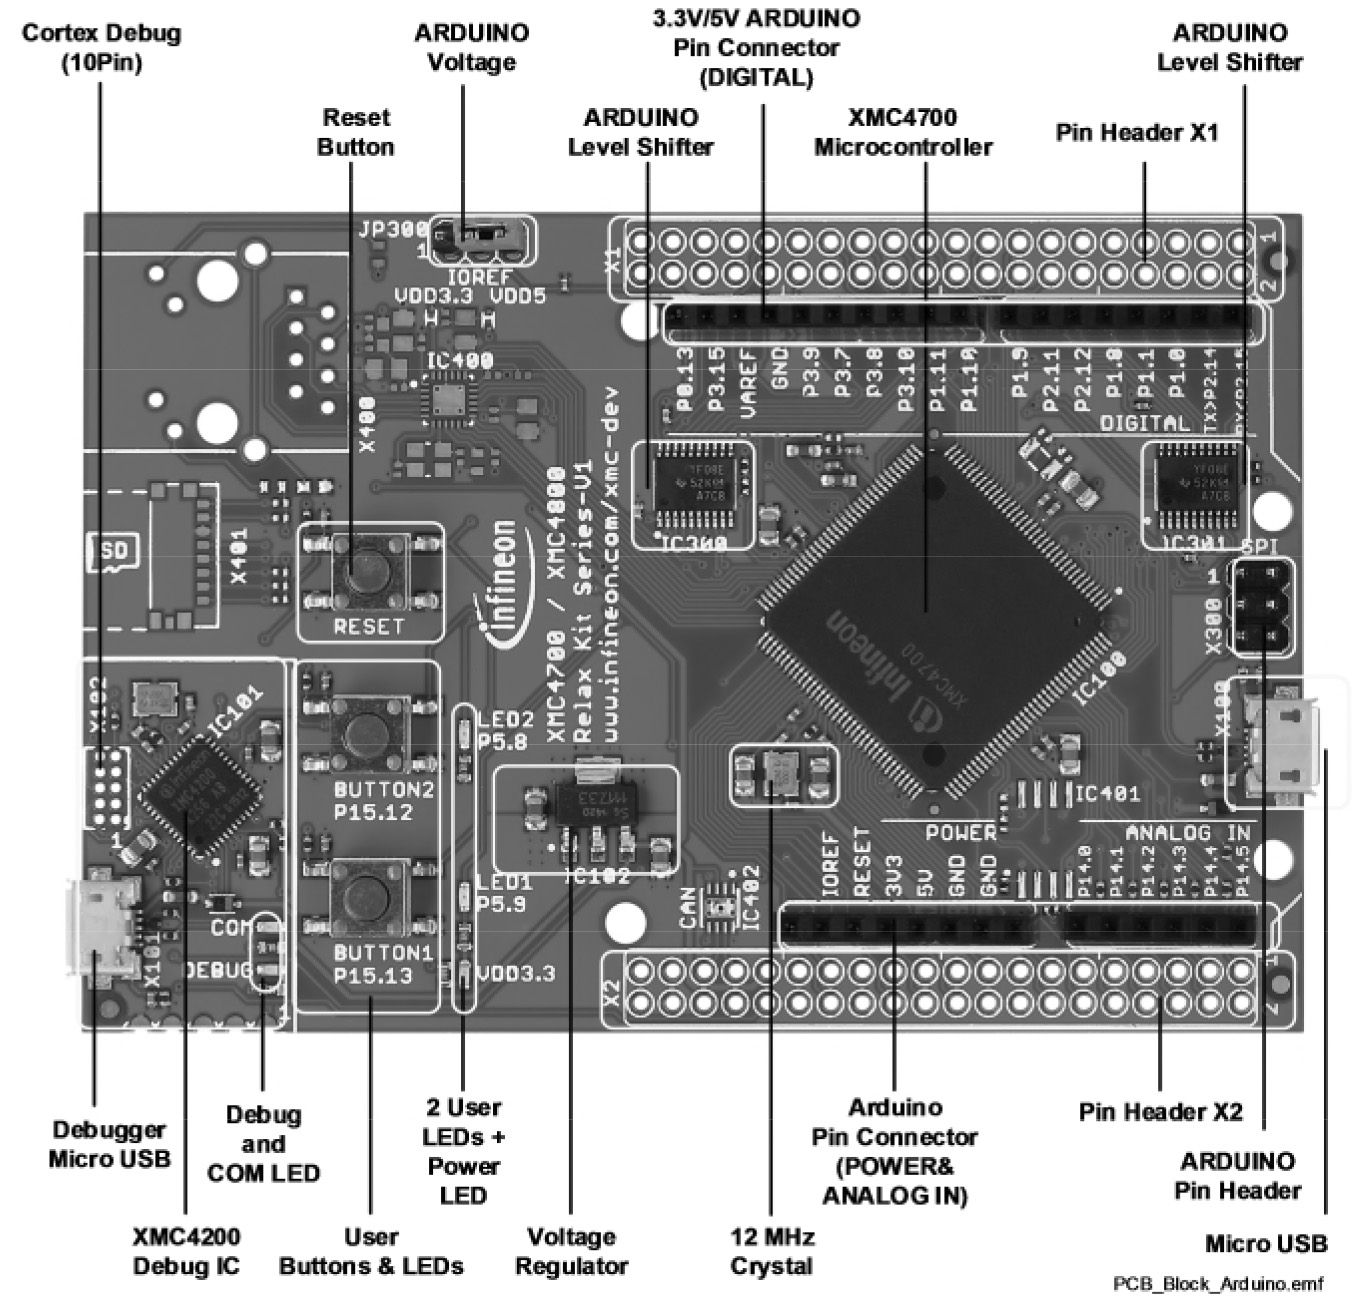
\includegraphics[width=\textwidth-6cm]{hardware/graphics/XMC_4700_Board_overview}
	\caption{XMC 4700 Relax Kit 5V}
	\quelle \url{http://www.infineon.com}
	%quelle http://www.infineon.com/export/sites/default/media/products/Microcontrollers/XMC/XMC4700_Relax_Kit.JPG_472149771.jpg
	\label{fig:XMC4700}	
\end{figure}

\paragraph{Bidirektionale Spannungswandler TXS0108}
Auf dem Relax Kit sind für die Pegelwandlung von 5 Volt zu 3.3 Volt zwei Levelshifter vom Typ TXS0108 aufgebracht.
Diese setzen einen angelegten Logischen Pegel von einer Quellspannung auf eine zweite um.
Dies kann bidirektional geschehen.
Dadurch ist es möglich die I/O Pins als Ein- oder Ausgang zu verwenden.

Ein Problem, dass während der Durchführung des Projektes auftrat war ein Schwingen bzw. ein Burst-Signal. 
Ursache hierfür waren zu lange Anschlussleitungen.
Der Hersteller, Texas Instruments, verweist in seinem Handbuch darauf, dass die Leitungslänge kurz gehalten werden muss um Reflexionen zu vermeiden.
Das Verhalten bei solchen Reflexionen wird nicht näher beschrieben.
Genaueres kann dem Abschnitt ??? entnommen werden.
Unter Normalbedingungen, damit ist die Verwendung der Levelshifter mit Arduino Shields gemeint, dürfte ein solches Problem nicht auftreten, da die Signalleitungen nur wenige Zentimeter betragen.

%----------------------------------------------------------------------------------


\subsection{XMC 4800 Relax EtherCat Kit}
\label{sec:XMC4800}
Dieses Kit entspricht, mit ein paar Unterschieden, dem XMC 4700 Relax Kit 5V.
Auf diesem Kit befinden sich keine Levelshifter.
Dies sind durch 0-Ohm Widerstände ersetzt.
In Abbildung \ref{fig:XMC4800} sind diese entsprechend markiert.
Dadurch ist die Verwendung von 5 Volt Arduino Shields nicht möglich.
Des weiteren ist bereits eine Anschlussbuchse für Ethernet und ein EtherCat Adapterboard vorhanden.
Bei EtherCat handelt es sich um eine echtzeitfähige Ethernet Kommunikation, die vorwiegend in der Automatisierungstechnik eingesetzt wird. 

\begin{figure}[hptb]
	\centering
	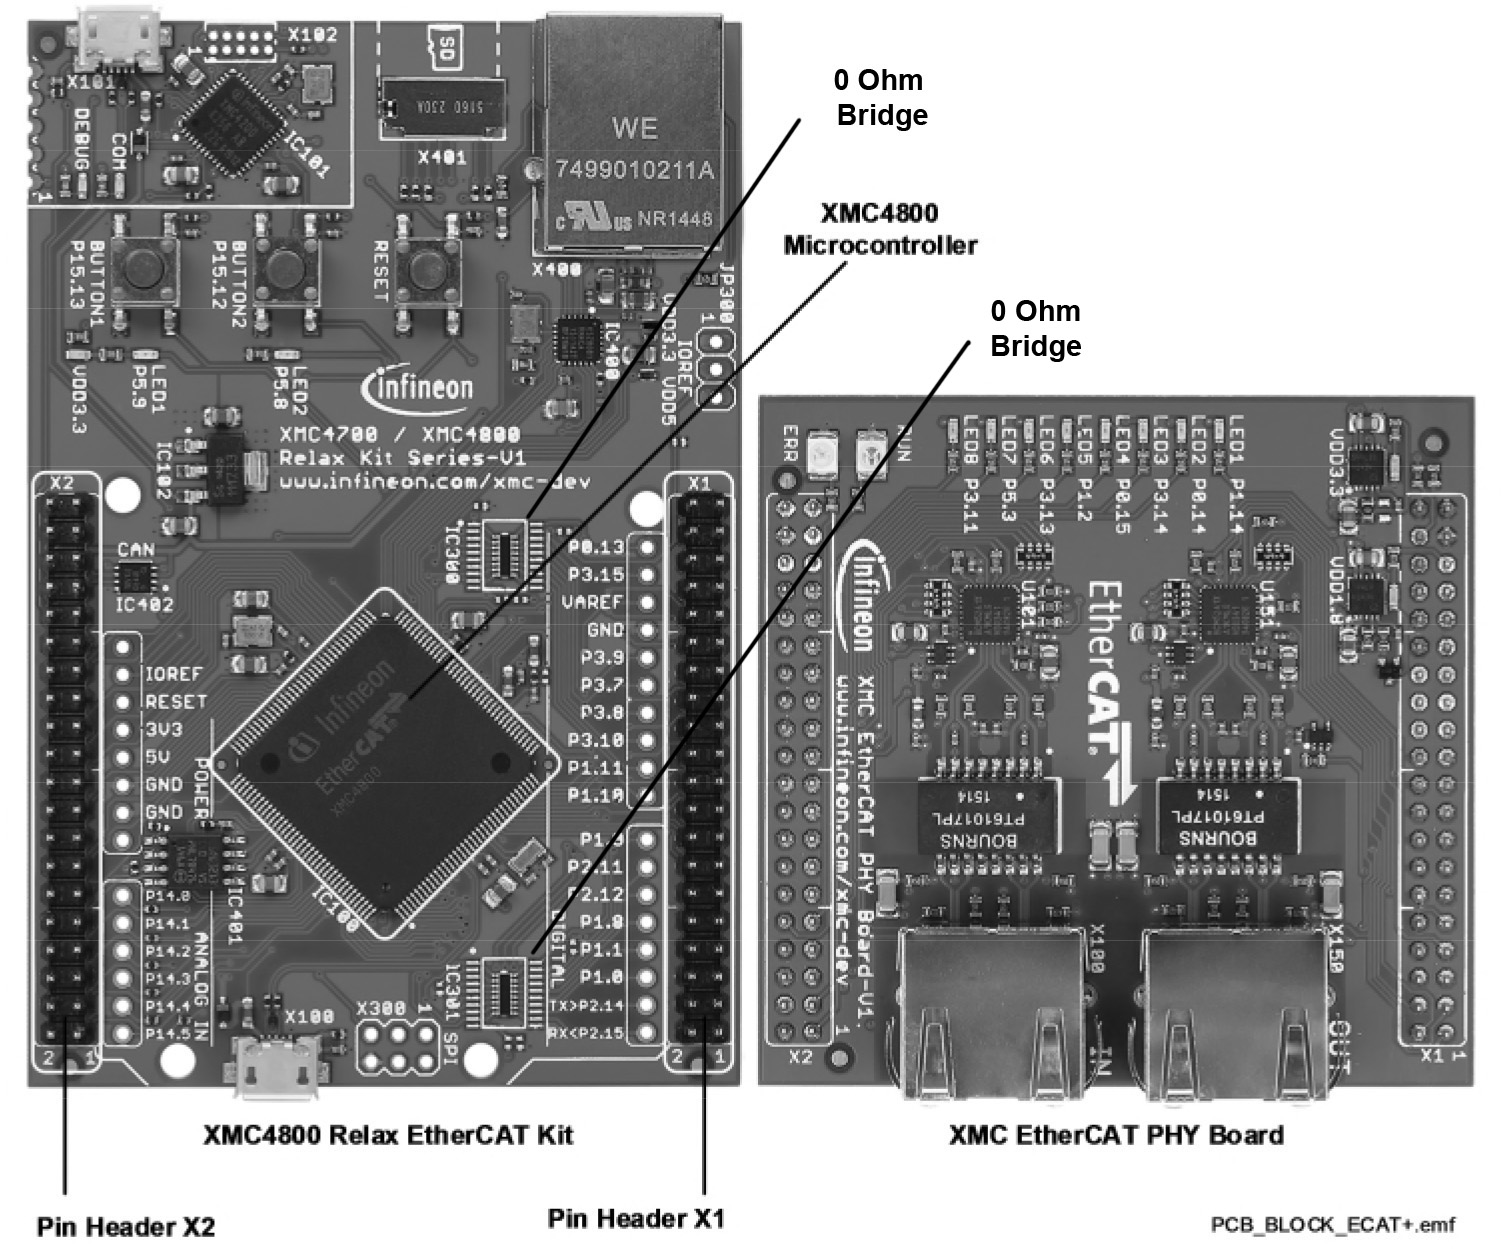
\includegraphics[width=\textwidth-4cm]{hardware/graphics/XMC_4800_Board_with_EtherCAT}
	\caption{XMC 4800 Relax Kit mit EtherCat PHY Board}
	\quelle http://www.infineon.com
	%quelle 
	\label{fig:XMC4800}
\end{figure}

%----------------------------------------------------------------------------------


\section{Texas Instrument DRV8302 Evaluation Kit}	
\label{sec:TI DRV8302 EvalKit}
Mit diesem Kit stellt Texas Instrument eine fertig Plattform für die Entwicklung von Motorsteuerungen und das Experimentieren mit BLDC-Motoren\footnote{BLDC ist die Kurzform für Brushless DC und bezeichnet den Grundlegenden Aufbau eines Motors.} zur Verfügung.
Es besteht aus dem Evaluation Board, Controller Karte, Anschlusskabeln und einer Steuerungssoftware für die Controller Karte (siehe Abbildung \ref{fig:DRV8302EvalKit}).
Damit ist es ohne großen Aufwand möglich BLDC-Motoren anzusteuern.
Über verschiedene, auf der Platine vorhandenen, Schutzmechanismen wie Überstrombegrenzung soll ein Zerstören des Angeschlossenen Motors verhindert werden.

\begin{figure}[h]
	\centering
	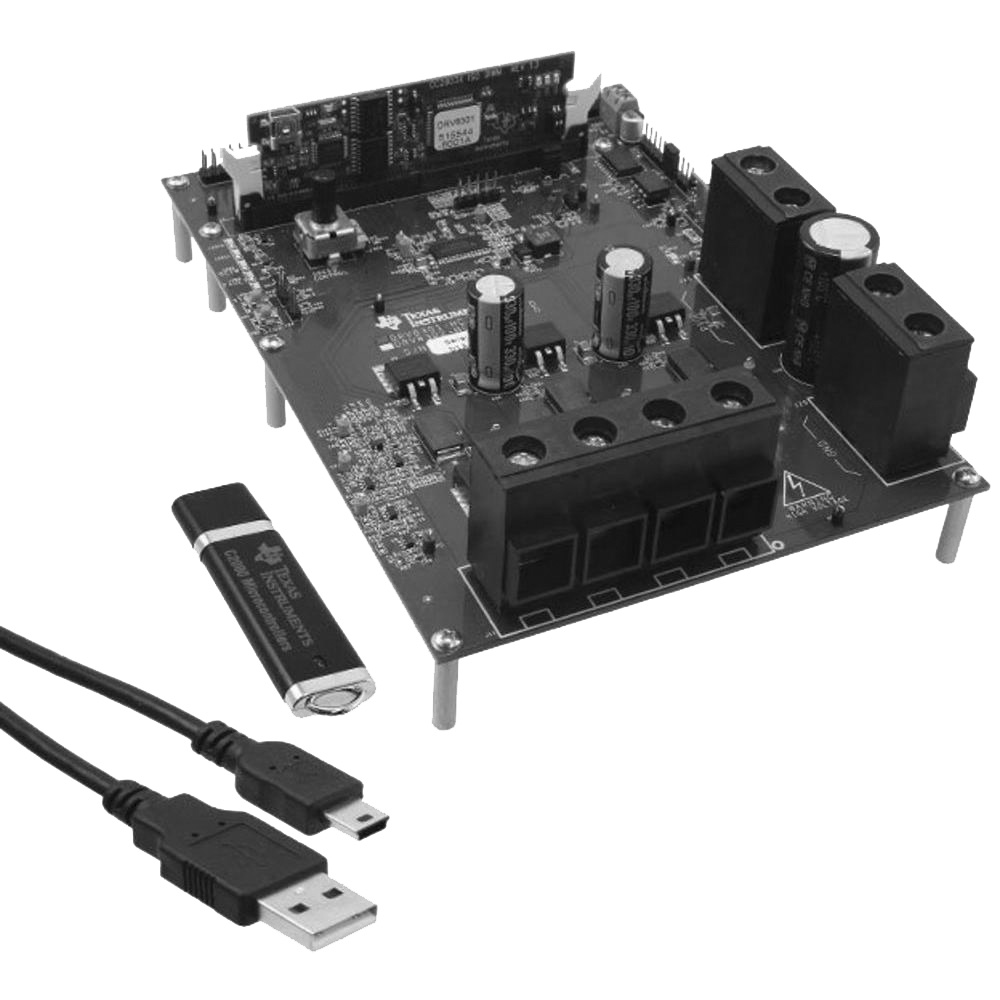
\includegraphics[width=8cm]{hardware/graphics/1189086_BB_00_FB}
	\caption[DRV8302 Evaluation Kit]{Texas Instrument DRV8302 Evaluation Kit}
	\quelle http://www.ti.com
	\label{fig:DRV8302EvalKit}
\end{figure}

In Abbildung \ref{fig:DRV8302Board} ist das Evaluation Board dargestellt.
Kernstück des Evaluation Boards ist ein Drei-Phasen-Treiberchip (DRV8302).
Dieser steuert die darunter liegenden Feldeffekttransistor, welche den Arbeitsstrom auf die verschiedenen Wicklungen des Motors schalten.
Der DRV8302 kann mit einer Spannung von 8 V bis 60 V Gleichspannung versorgt werden.
Die Leistungstransistoren können eine Spitzenstrom von 60 A pro Phase schalten.
Am unteren Ende der Platine befindet sich das Anschlussterminal für den Motor.
Rechts daneben das für die Versorgungsspannung.

\begin{figure}[htbp]
	\centering
	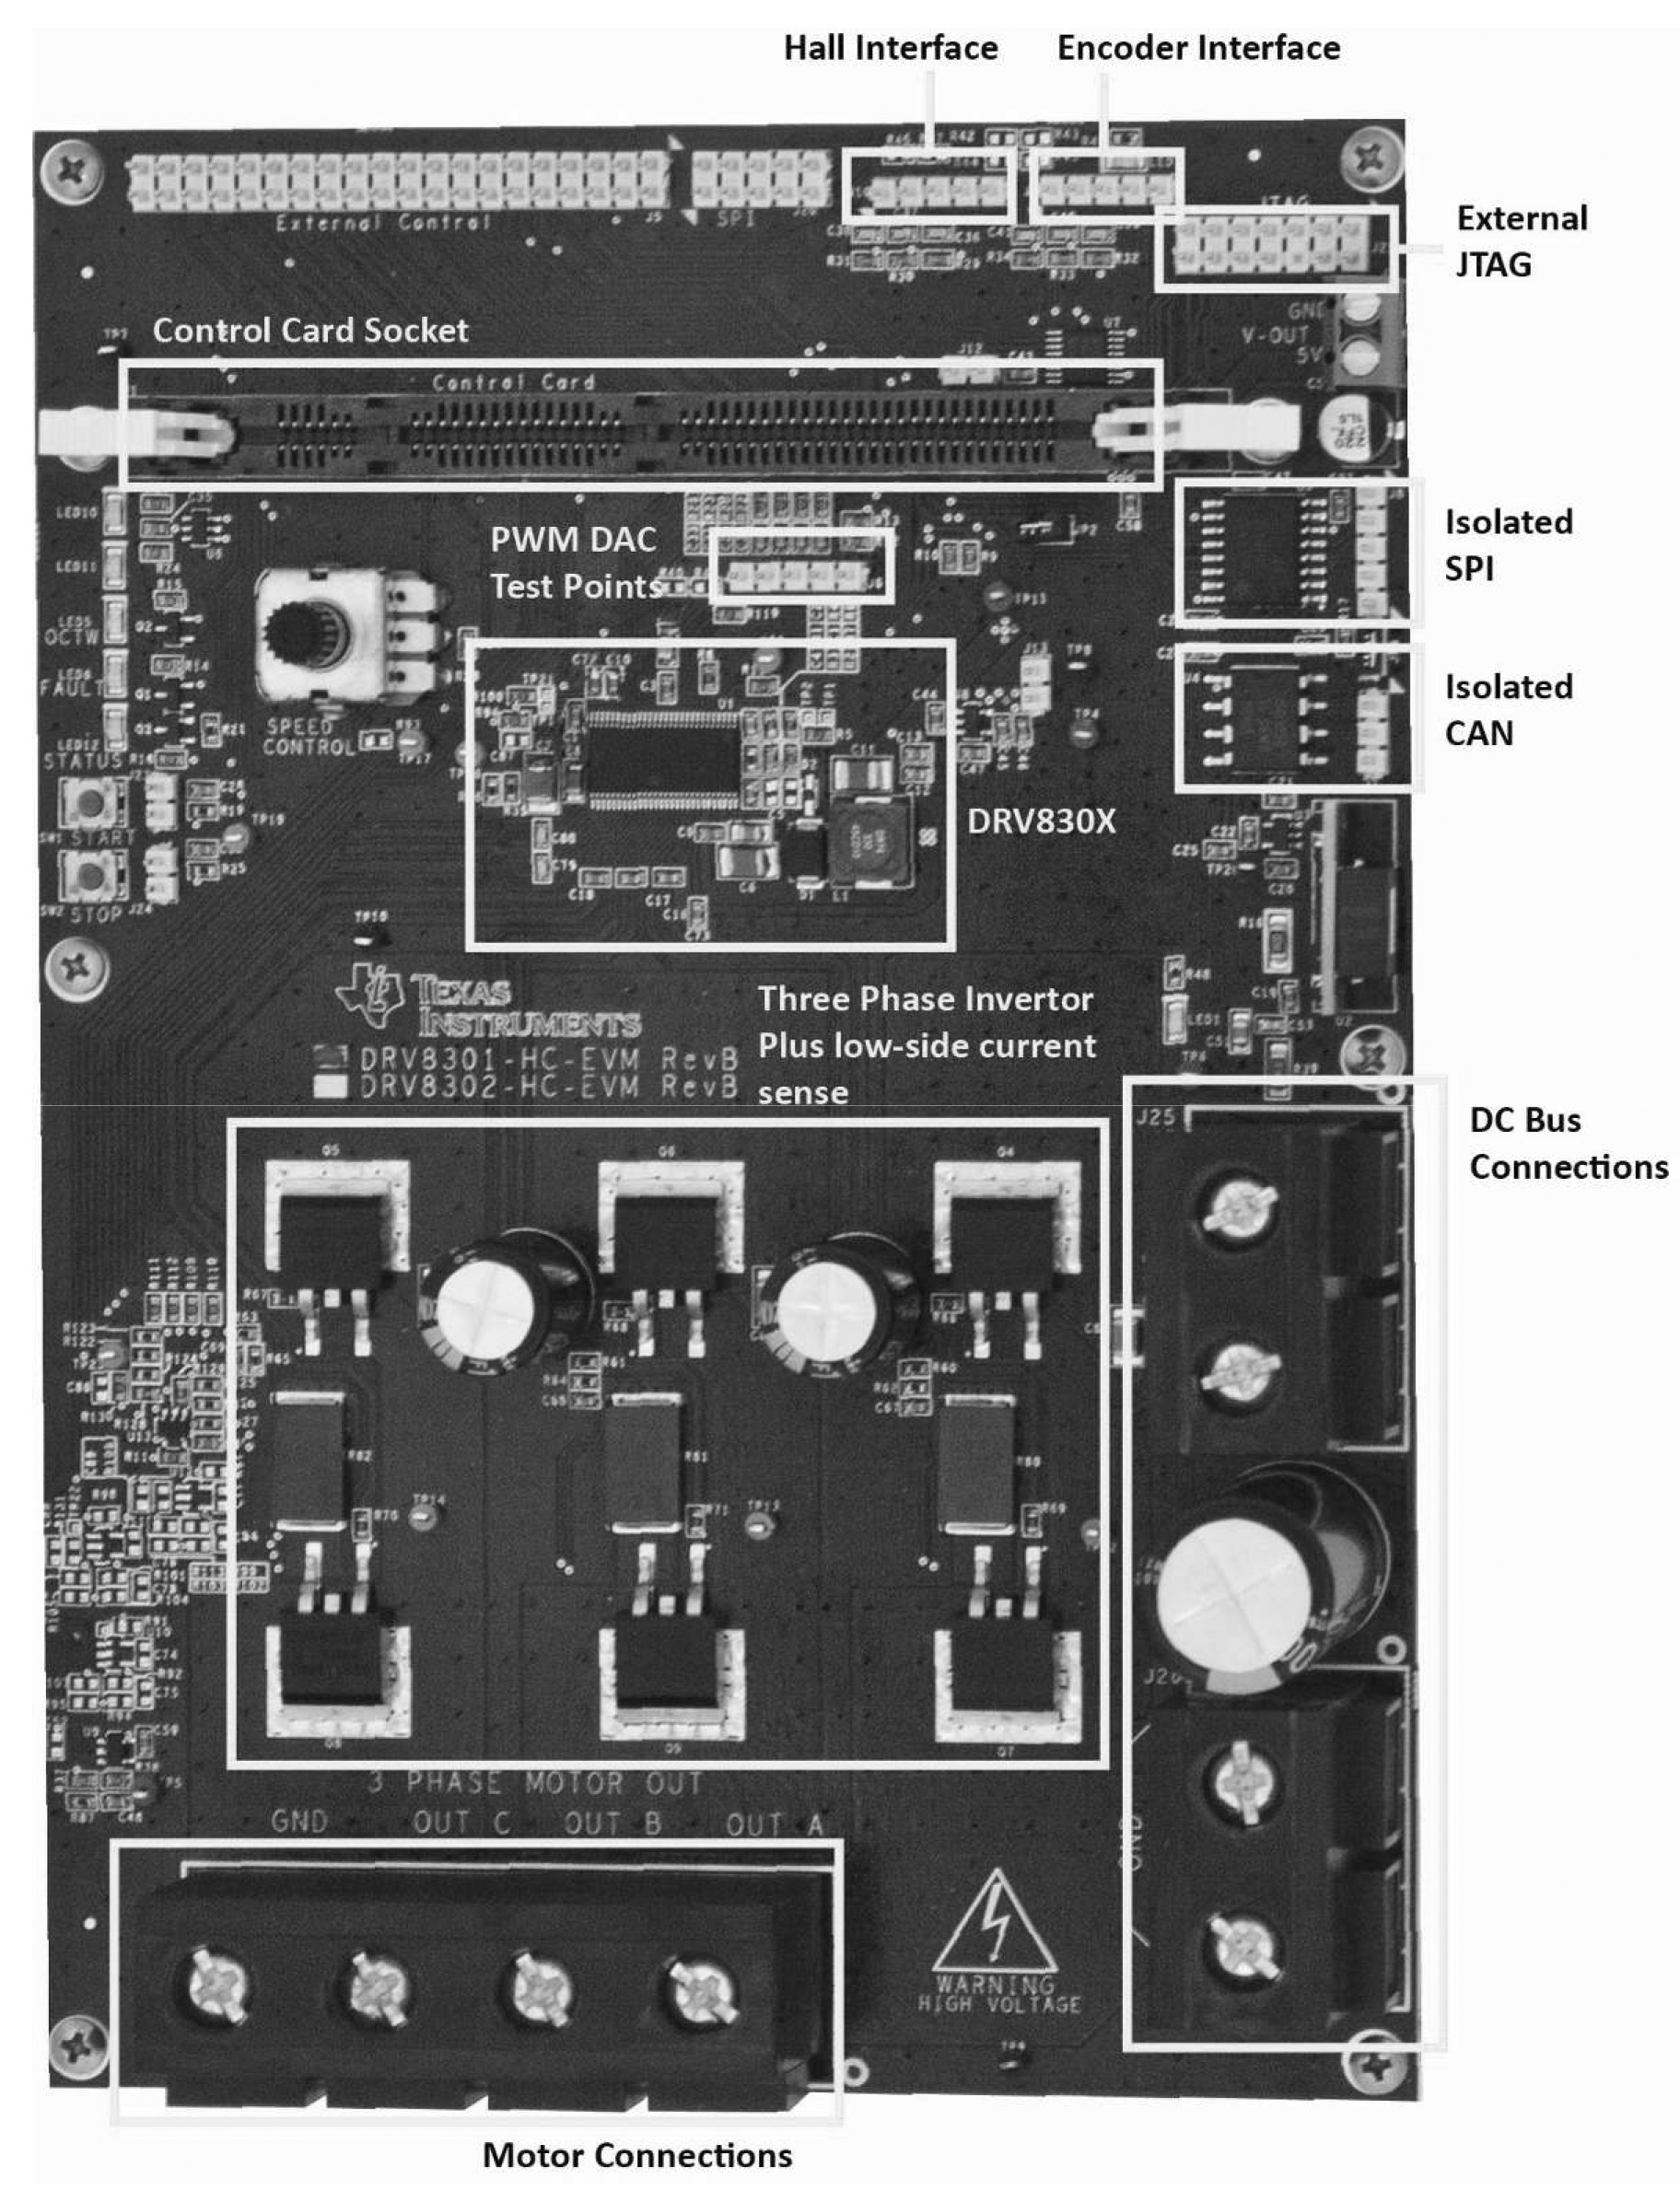
\includegraphics[width=\textwidth]{hardware/graphics/TI_Eval_Board}
	\caption{DRV8302 Evaluation Board}
	\quelle \cite{Instruments2014}
	\label{fig:DRV8302Board}
\end{figure}

%----------------------------------------------------------------------------------

\section{PMD-BLDC-1500/65}
Als Motor für den Experimentierplatz wird ein Bürstenloser Gleischstrommotor eingesetzt (kurz BLDC), genauer gesagt ein LRK Motor. 
Benannt ist dieser nach den drei Person, die an seiner Entwicklung beteiligt waren.
Christian \textbf{L}ukas hatte Ende 2000 die Idee von diesen Motoren, die Ludwig \textbf{R}etzbach in der Elektro-Modell veröffentlichte, und Herr \textbf{K}ühfuß die ersten Drehteile herstellte.
%quelle http://www.torquemax.de/Motoren/default.html
Der allgemeine Vorteil von Bürstenlosen Motoren liegt darin, dass es keine Verschleißteile gibt.
Hingegen müssen bei klassischen Gleichstrommotoren mit Bürsten diese ersetzt werden sobald sie verbraucht oder zerstört sind.
Für die Regelung des Motors sind drei digitale Hall-Sensoren verbaut.
Zur Temperaturüberwachung ist ein NTC-Sensor innerhalb des Motors angebracht. 
NTC ist hierbei die Kurzform für Negative Temperature Coefficient Thermistor und beschreibt einen Temperaturabhängigen Widerstand.
Dieser verringert seinen Widerstand bei steigender Temperatur.
